\documentclass[12pt,titlepage,letterpaper]{article}

\usepackage{hw}

\title{Homework I}
\author{Hanlin He (hxh160630)}
\date{\today}

\begin{document}
\maketitle

\section{IP Addressing and Subnetting}
\begin{enumerate}[label=\bfseries\alph*)]
    \item To configure B and C as a subnet, it takes at least two available IP
        address, plus the reserve address for broadcast and the subnet itself.
        So it would be a subnet with subnet mask of \texttt{30}, or in
        dot-decimal notation of \texttt{255.255.255.252}. In conclusion, the
        number of addresses available for the Ethernet would be reduced by
        four.
    \item As ARP proxy, B would pretend to be C in front of A.
        \begin{enumerate}[label=\bfseries\roman*. ]
            \item Packets send sequence would be like \cref{1ai}.
                \begin{table}[H]
                \footnotesize
                \centering
                \caption{All Packets Sent}\label{1ai}
                \begin{tabular}{c|c|c|c|c|c}
                    Message & \multirow{2}{*}{Sender} & Sender's & Sender's &
                    Target & Target \\
                    Type & & MAC Addr & IP Addr & MAC Addr & IP Addr \\\hline\hline
                    ARP Req & A & A's MAC addr & A's IP & 00-00-00-00-00-00 &
                    C's IP \\
                    ARP reply & B & B's MAC addr & C's IP & A's MAC addr &
                    A's IP \\%\hline
                    %&&&&&\\
                    IP msg & A & A's MAC addr & A's IP & B's MAC addr &
                    C's IP 
                \end{tabular}
                \end{table}
            \item To implement the proxy ARP, B's routing table need to add
                rules that for for all received or generated packets
                destination at C's IP address, the packets would go through the
                WIFI interface. And for packets received from C with
                destination address not B, B would forward the message to the
                Ethernet interface.
        \end{enumerate}
\end{enumerate}

\section{CIDR}
If the router actually containing that subset failed, the connected router
would detect that the link become unavailable and delete the ``correct''
routing policy. In the meantime, all the packets with the destination of that
subset addresses would be forwarded to the router advertising the ``big''
address blocks, since it's the only matching one, which lead to the wrong
domain.

\section{Internet Basics}
\begin{enumerate}[label=\bfseries\alph*)]
    \item The core router need to know the actual network number since the
        router still based on the routing table to forward a packet. Because
        the packet only contains a destination IP address, it does not contain
        the AS number it wants to go to. In other word, BGP only helps the
        router to build the routing table, it do not generate its own
        forwarding table.
    \item In theory, network administrator could redistribute all of the EBGP
        routes into the IGP. However, this is not recommended because of the
        large number of EBGP routes in the real Internet might cause the IGP
        crashes. By setting up iBGP among routers within an AS, and inject a
        default route (or boarder router pretend to have direct link with
        destination), the internal router could learn the best border router to
        use when sending a packet to any address.
    \item Firstly, advertising the entire AS-path would make routing loop
        easily detected. Secondly, sometimes network administrator might want
        the network traffic go through specific path due to some policy
        decisions. Only by know the entire AS-path can such requirement be
        fulfilled.
    \item 
\end{enumerate}

\section{Routing Policies}
\begin{enumerate}[label=\bfseries\alph*)]
    \item \texttt{E} would be willing to accept advertisement from \texttt{D}
        to maximize its monetary. Since if \texttt{E} accept from \texttt{B},
        it would increase expenses. And if \texttt{E} accept from \texttt{C},
        there will be no profit, since \texttt{C} is a peer.
    \item To enforce \texttt{E} accept advertisement from \texttt{C}, network
        administrator could set up a higher local preference.
    \item \texttt{E} would prefer \texttt{A} to use AS level path
        $\mathtt{A}\rightarrow\mathtt{D}\rightarrow\mathtt{E}$. Because
        receiving traffic from \texttt{D} would increase profit via providing
        service to \texttt{D}.
    \item To cause the traffic to propagate on path 
        $\mathtt{A}\rightarrow\mathtt{D}\rightarrow\mathtt{E}$, \texttt{E} can
        prepend its AS path towards \texttt{B} and \texttt{C} to make the path
        longer. That is, instead of advertising AS path \texttt{[E]},
        \texttt{E} can advertising a longer AS path \texttt{[E,E]} to both
        \texttt{B} and \texttt{C}, and advertising the original AS path to
        \texttt{D}. By doing this, \texttt{A} would receive AS paths as:
        \begin{itemize}
            \item \texttt{[B,E,E]} from \texttt{B},
            \item \texttt{[C,E,E]} from \texttt{C},
            \item \texttt{[D,E]} from \texttt{D}.
        \end{itemize}
        \texttt{A} would choose the shorter one,
        $\mathtt{A}\rightarrow\mathtt{D}\rightarrow\mathtt{E}$.
    \item \texttt{B}, \texttt{C} and \texttt{D} should have at least the same
        local preference at AS \texttt{A}.\\ If, otherwise, local preference of
        \texttt{D} is lower, path
        $\mathtt{A}\rightarrow\mathtt{D}\rightarrow\mathtt{E}$
        would be discarded in the first place.
\end{enumerate}

\section{Dispute Graphs}
\begin{enumerate}[label=\bfseries\alph*)]
    \item The dispute graph for the system is shown in \cref{51}.
        \begin{figure}[H]
            \centering
            \caption{Dispute Graph for Original System}\label{51}
            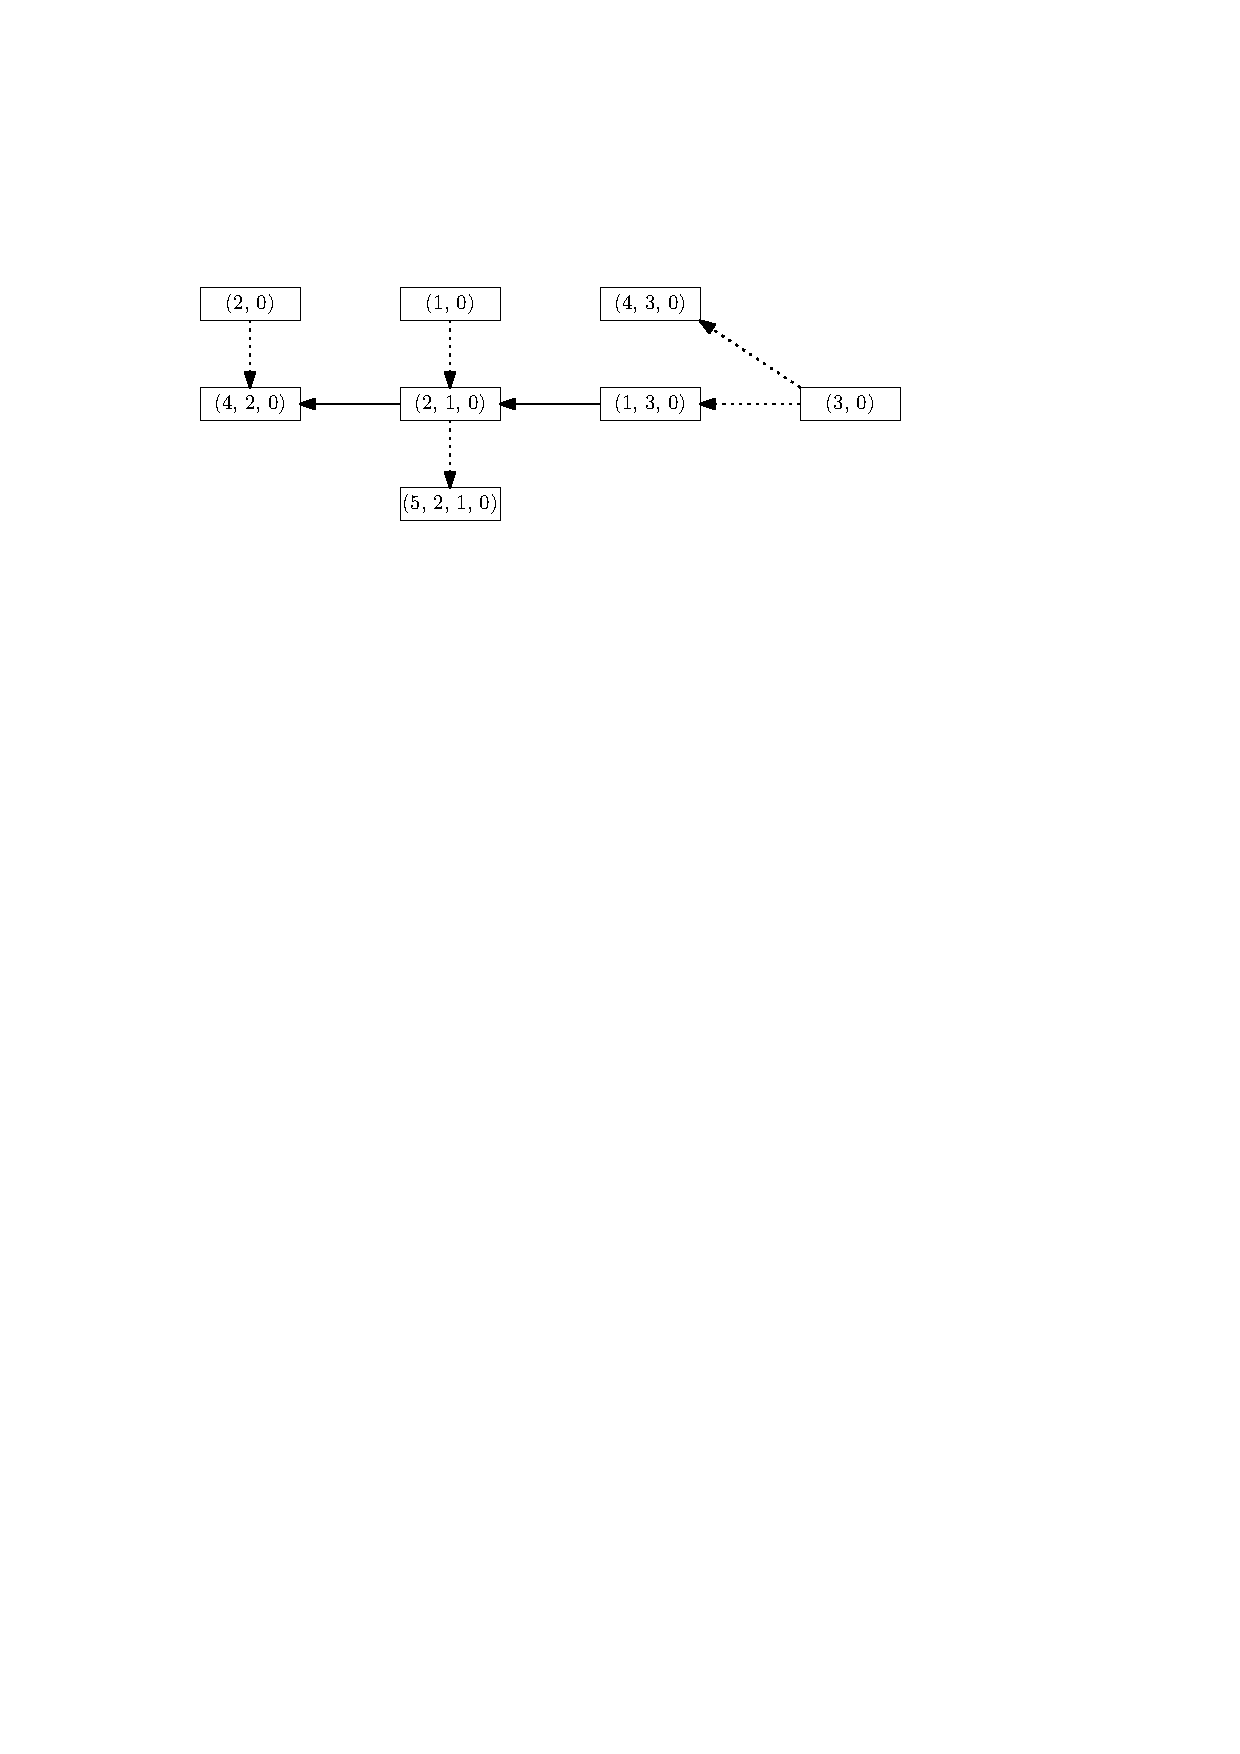
\includegraphics[width=.8\textwidth]{51}
        \end{figure}
    \item The dispute graph for the new system is shown in \cref{52}.
        \begin{figure}[H]
            \centering
            \caption{Dispute Graph for New System}\label{52}
            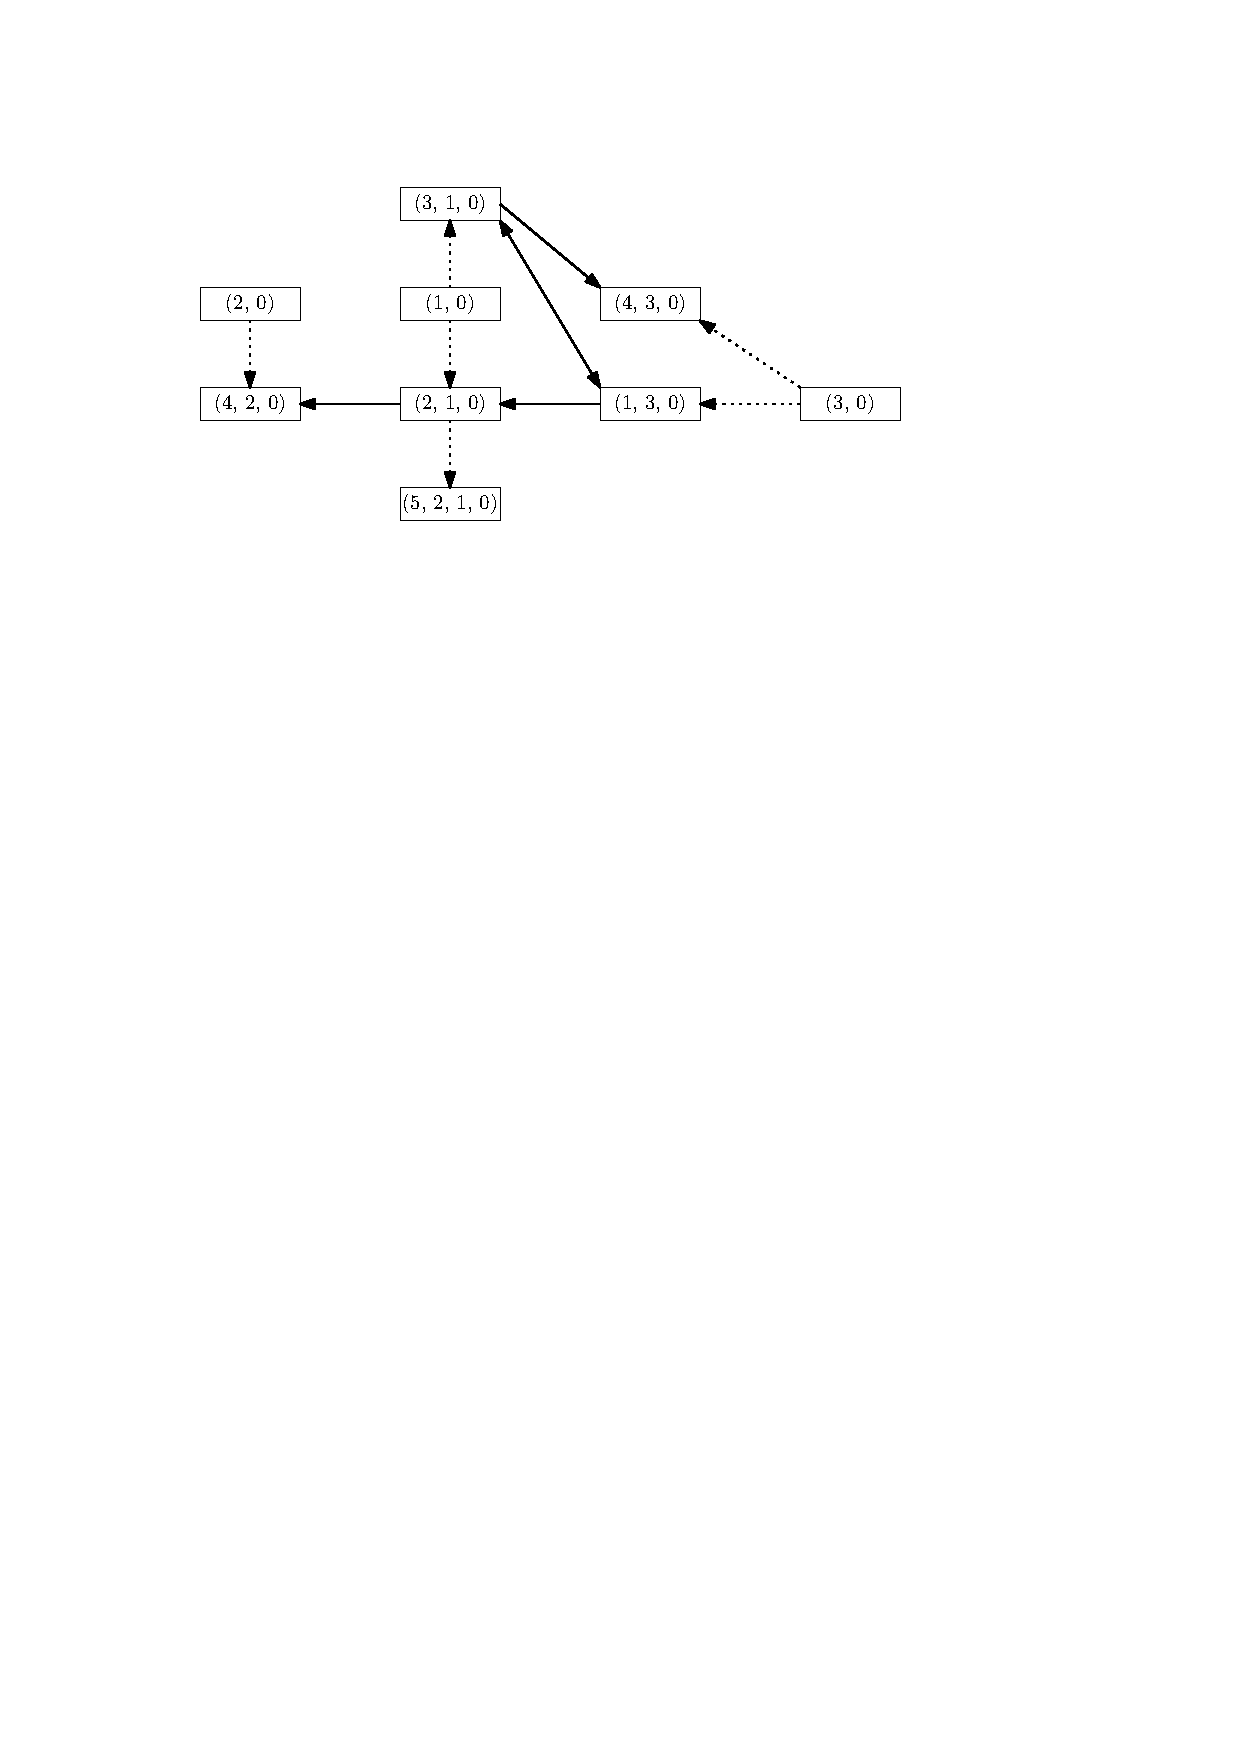
\includegraphics[width=.8\textwidth]{52}
        \end{figure}
    \item
        \begin{enumerate}[label=\roman*. ]
            \item After adding path $[3,1,0]$ to the system, AS0, AS1 and AS3
                became a \textsc{Disagree}.
                Since the rest of the system contains no dispute cycle,
                based on the \textsc{Disagree} we know that
                the system have two stable state as shown in \cref{53}.
                \begin{figure}[H]
                    \centering
                \caption{Two Stable State of the System}\label{53}
                    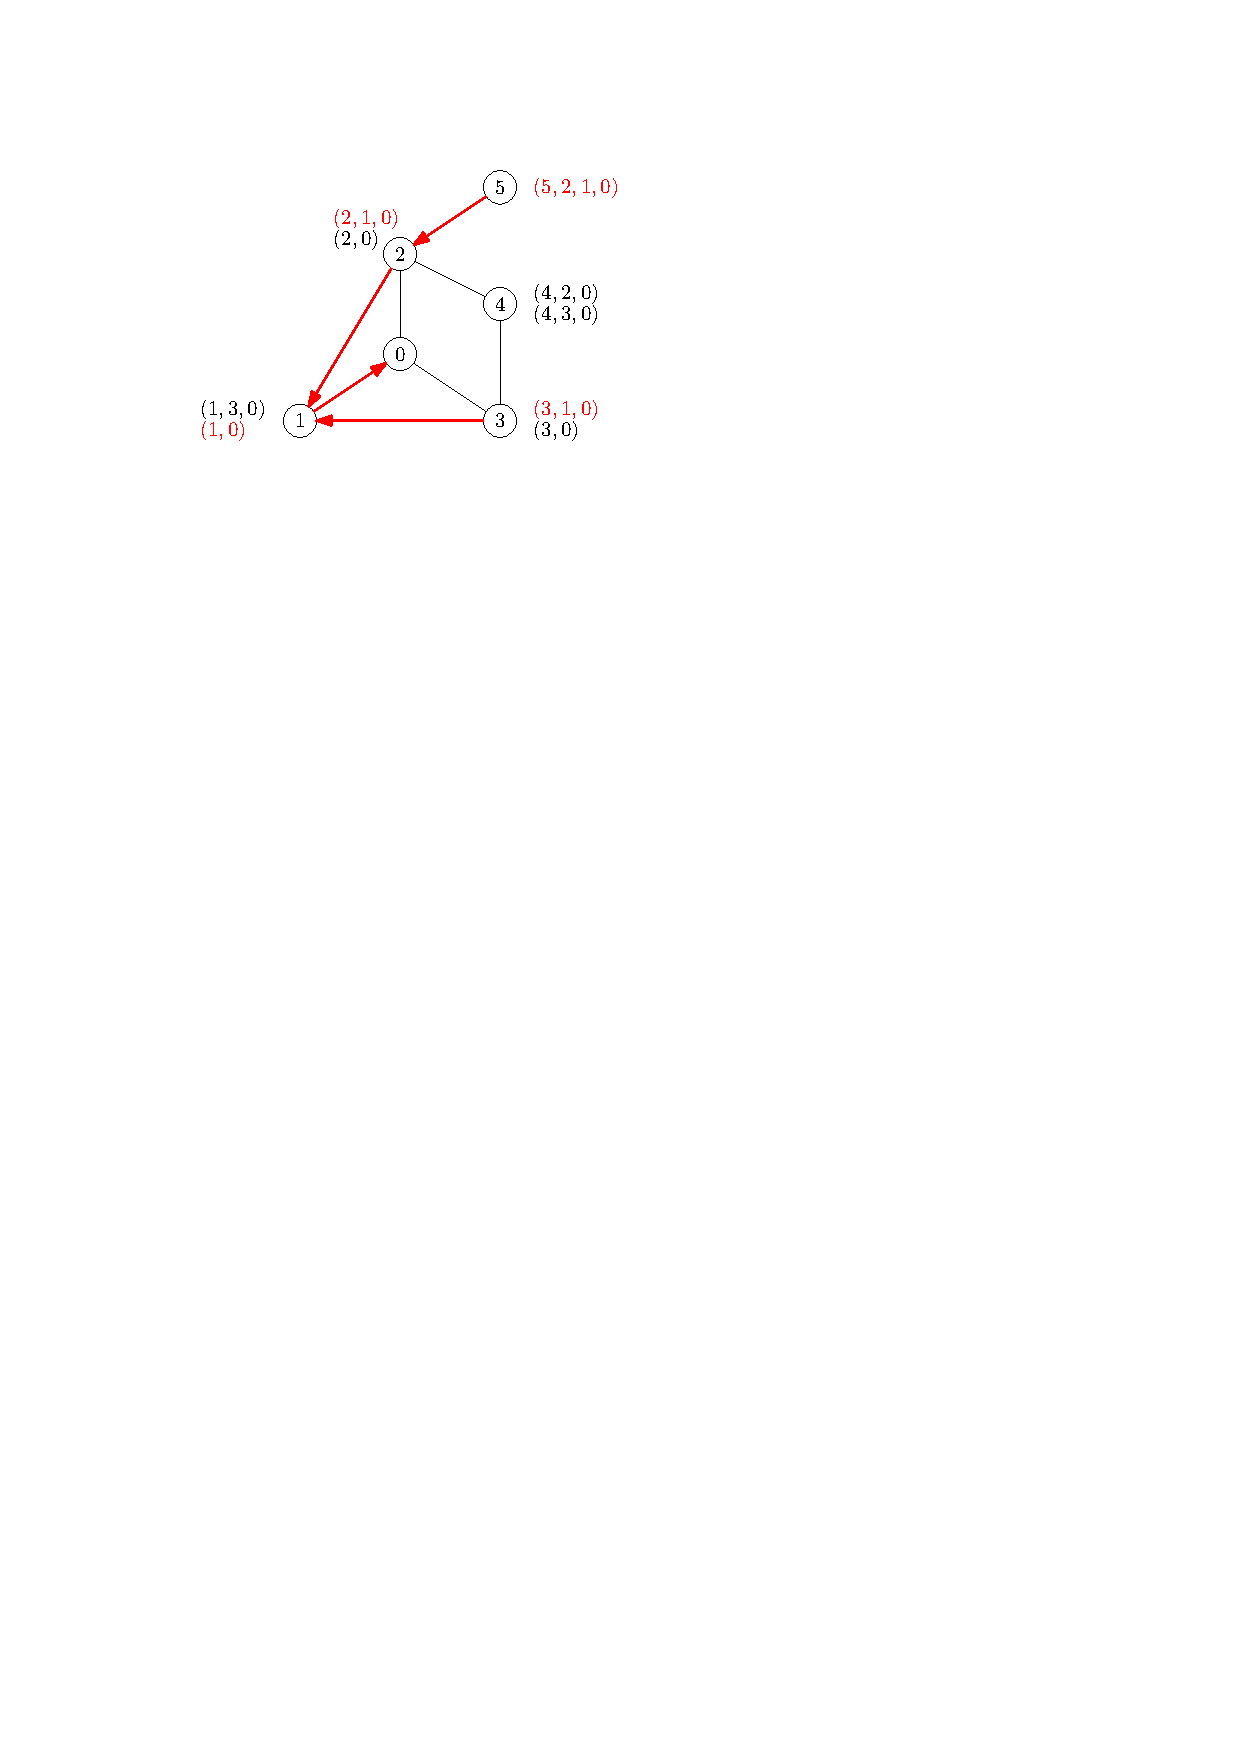
\includegraphics[width=.45\textwidth]{531}
                    \hfill
                    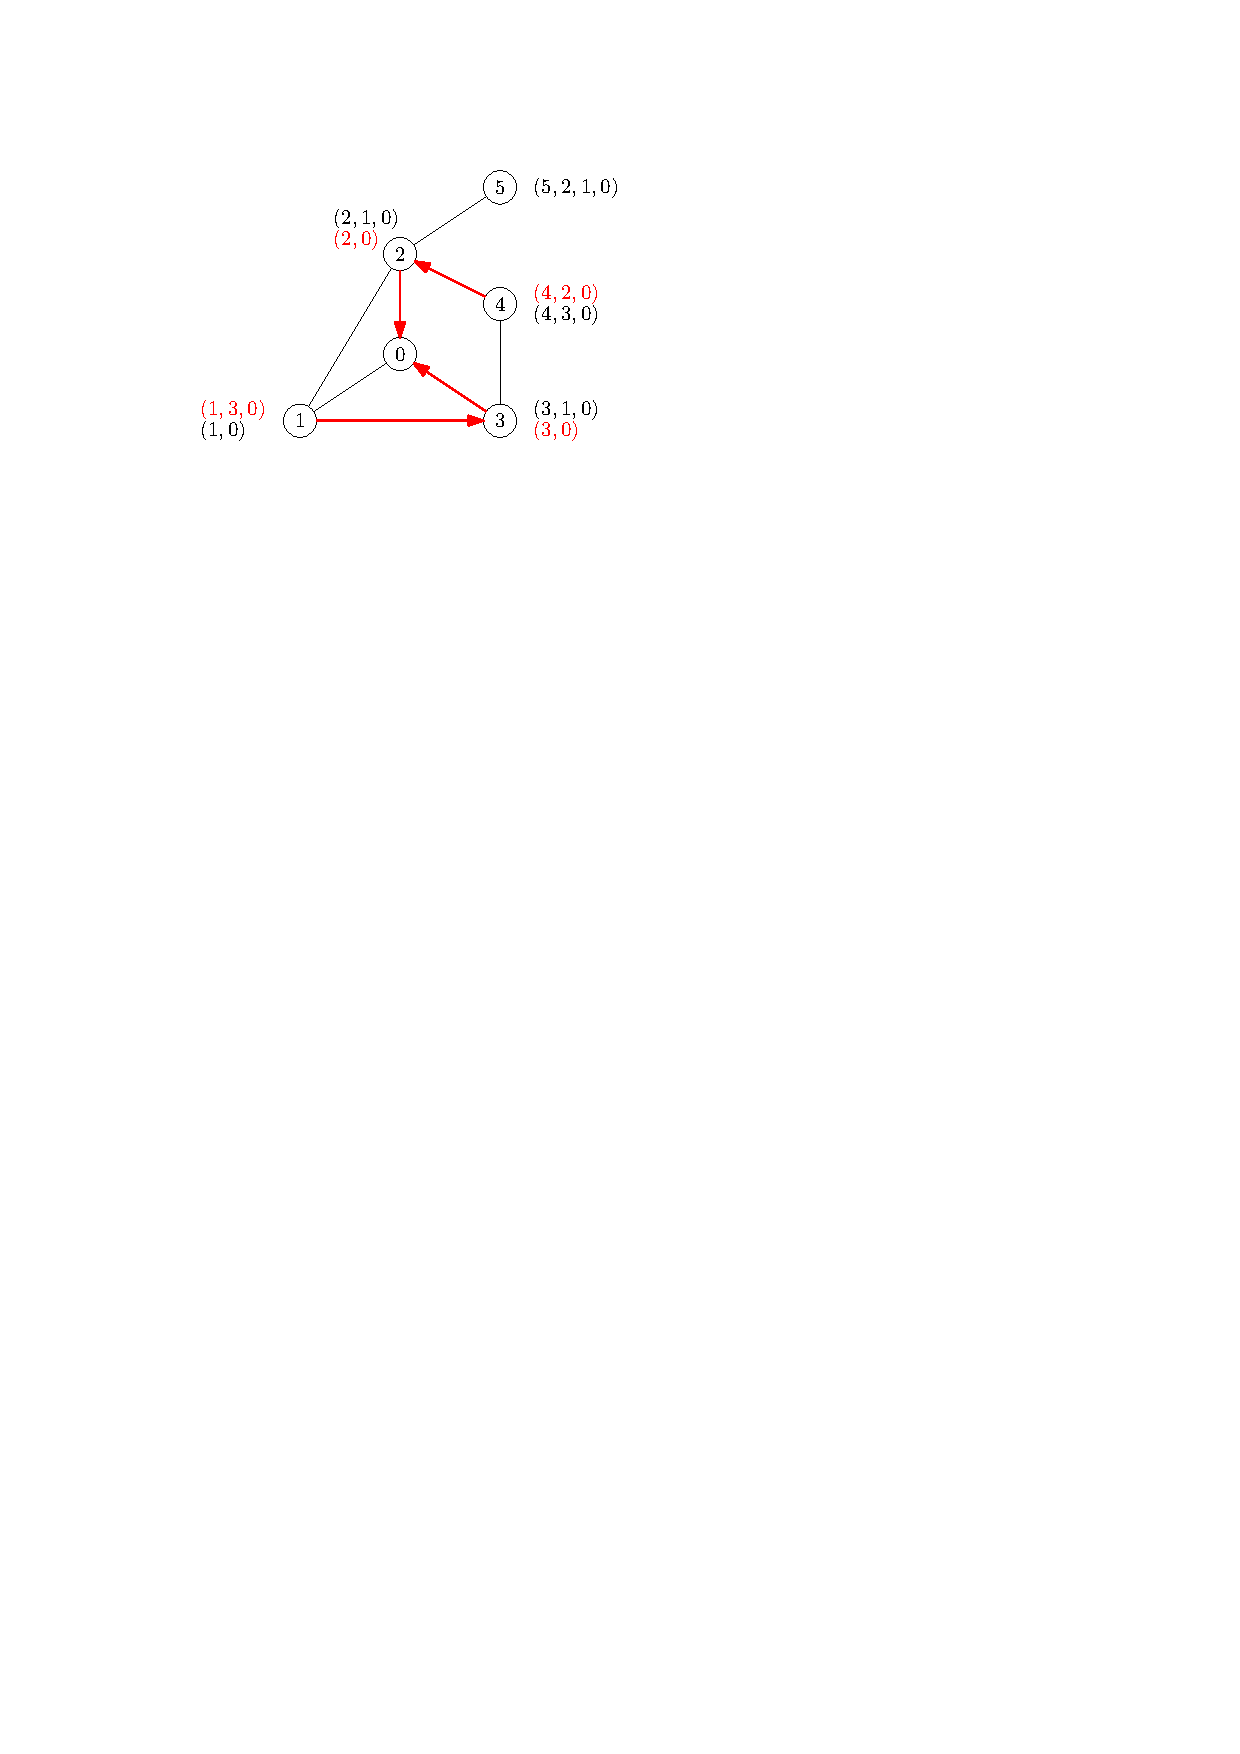
\includegraphics[width=.45\textwidth]{532}
                \end{figure}
            \item The system would always converge.\\
                We know that a \textsc{Disagree} would converge even though it
                contains a dispute cycle(wheel). And the system now has no
                dispute cycle(wheel) other than the \textsc{Disagree}.
                Thus, we can conclude that the system would always converge.
        \end{enumerate}
\end{enumerate}

\section{Hierarchical BGP}

\section{Ethernet Multicast}

\section{Reverse Path Flooding}

\section{DVMRP}

\end{document}
